En esta sección se presentan y analizan los resultados empíricos obtenidos en las pruebas de rendimiento. Cada punto graficado corresponde al promedio aritmético de las tres réplicas independientes ($a, b, c$) ejecutadas para cada configuración experimental.

\subsection{Resultados en Algoritmos de Ordenamiento}

El módulo de ordenamiento evalúa el tiempo de ejecución en función del tamaño del arreglo $N \in [10^1, 10^7]$ combinando distintas distribuciones iniciales y dominios numéricos. 

Para apreciar resultados se muestran las tres distribuciones evaluadas bajo el dominio amplio $D_7$ (aleatorio, descendente y ascendente). El motivo de esta decisión es debido a que: en $D_7$ los números casi no se repiten, lo que evita atajos accidentales por valores duplicados y permite aislar los comportamientos más interesantes y realistas del experimento:
\begin{itemize}
    \item Algoritmos como \textit{Merge Sort} y \textit{std::sort} son prácticamente insensibles a la forma de la entrada: \textit{Merge Sort} siempre divide el arreglo en mitades iguales ejecutando un costo constante de división y mezcla, y asumimos que \textit{std::sort} es sumamente robusto debido a las optimizaciones internas de la biblioteca estándar de C++. Ambos mantienen siempre su tendencia esperada $\mathcal{O}(N \log N)$.
    \item Pero notamos que, \textit{Quick Sort} y \textit{Patience Sort} son los métodos que exhiben variaciones frente al orden inicial de los datos, justificando un análisis detallado de sus casos extremos.
\end{itemize}

\begin{figure}[htbp]
    \centering
    \begin{minipage}{0.48\textwidth}
        \centering
        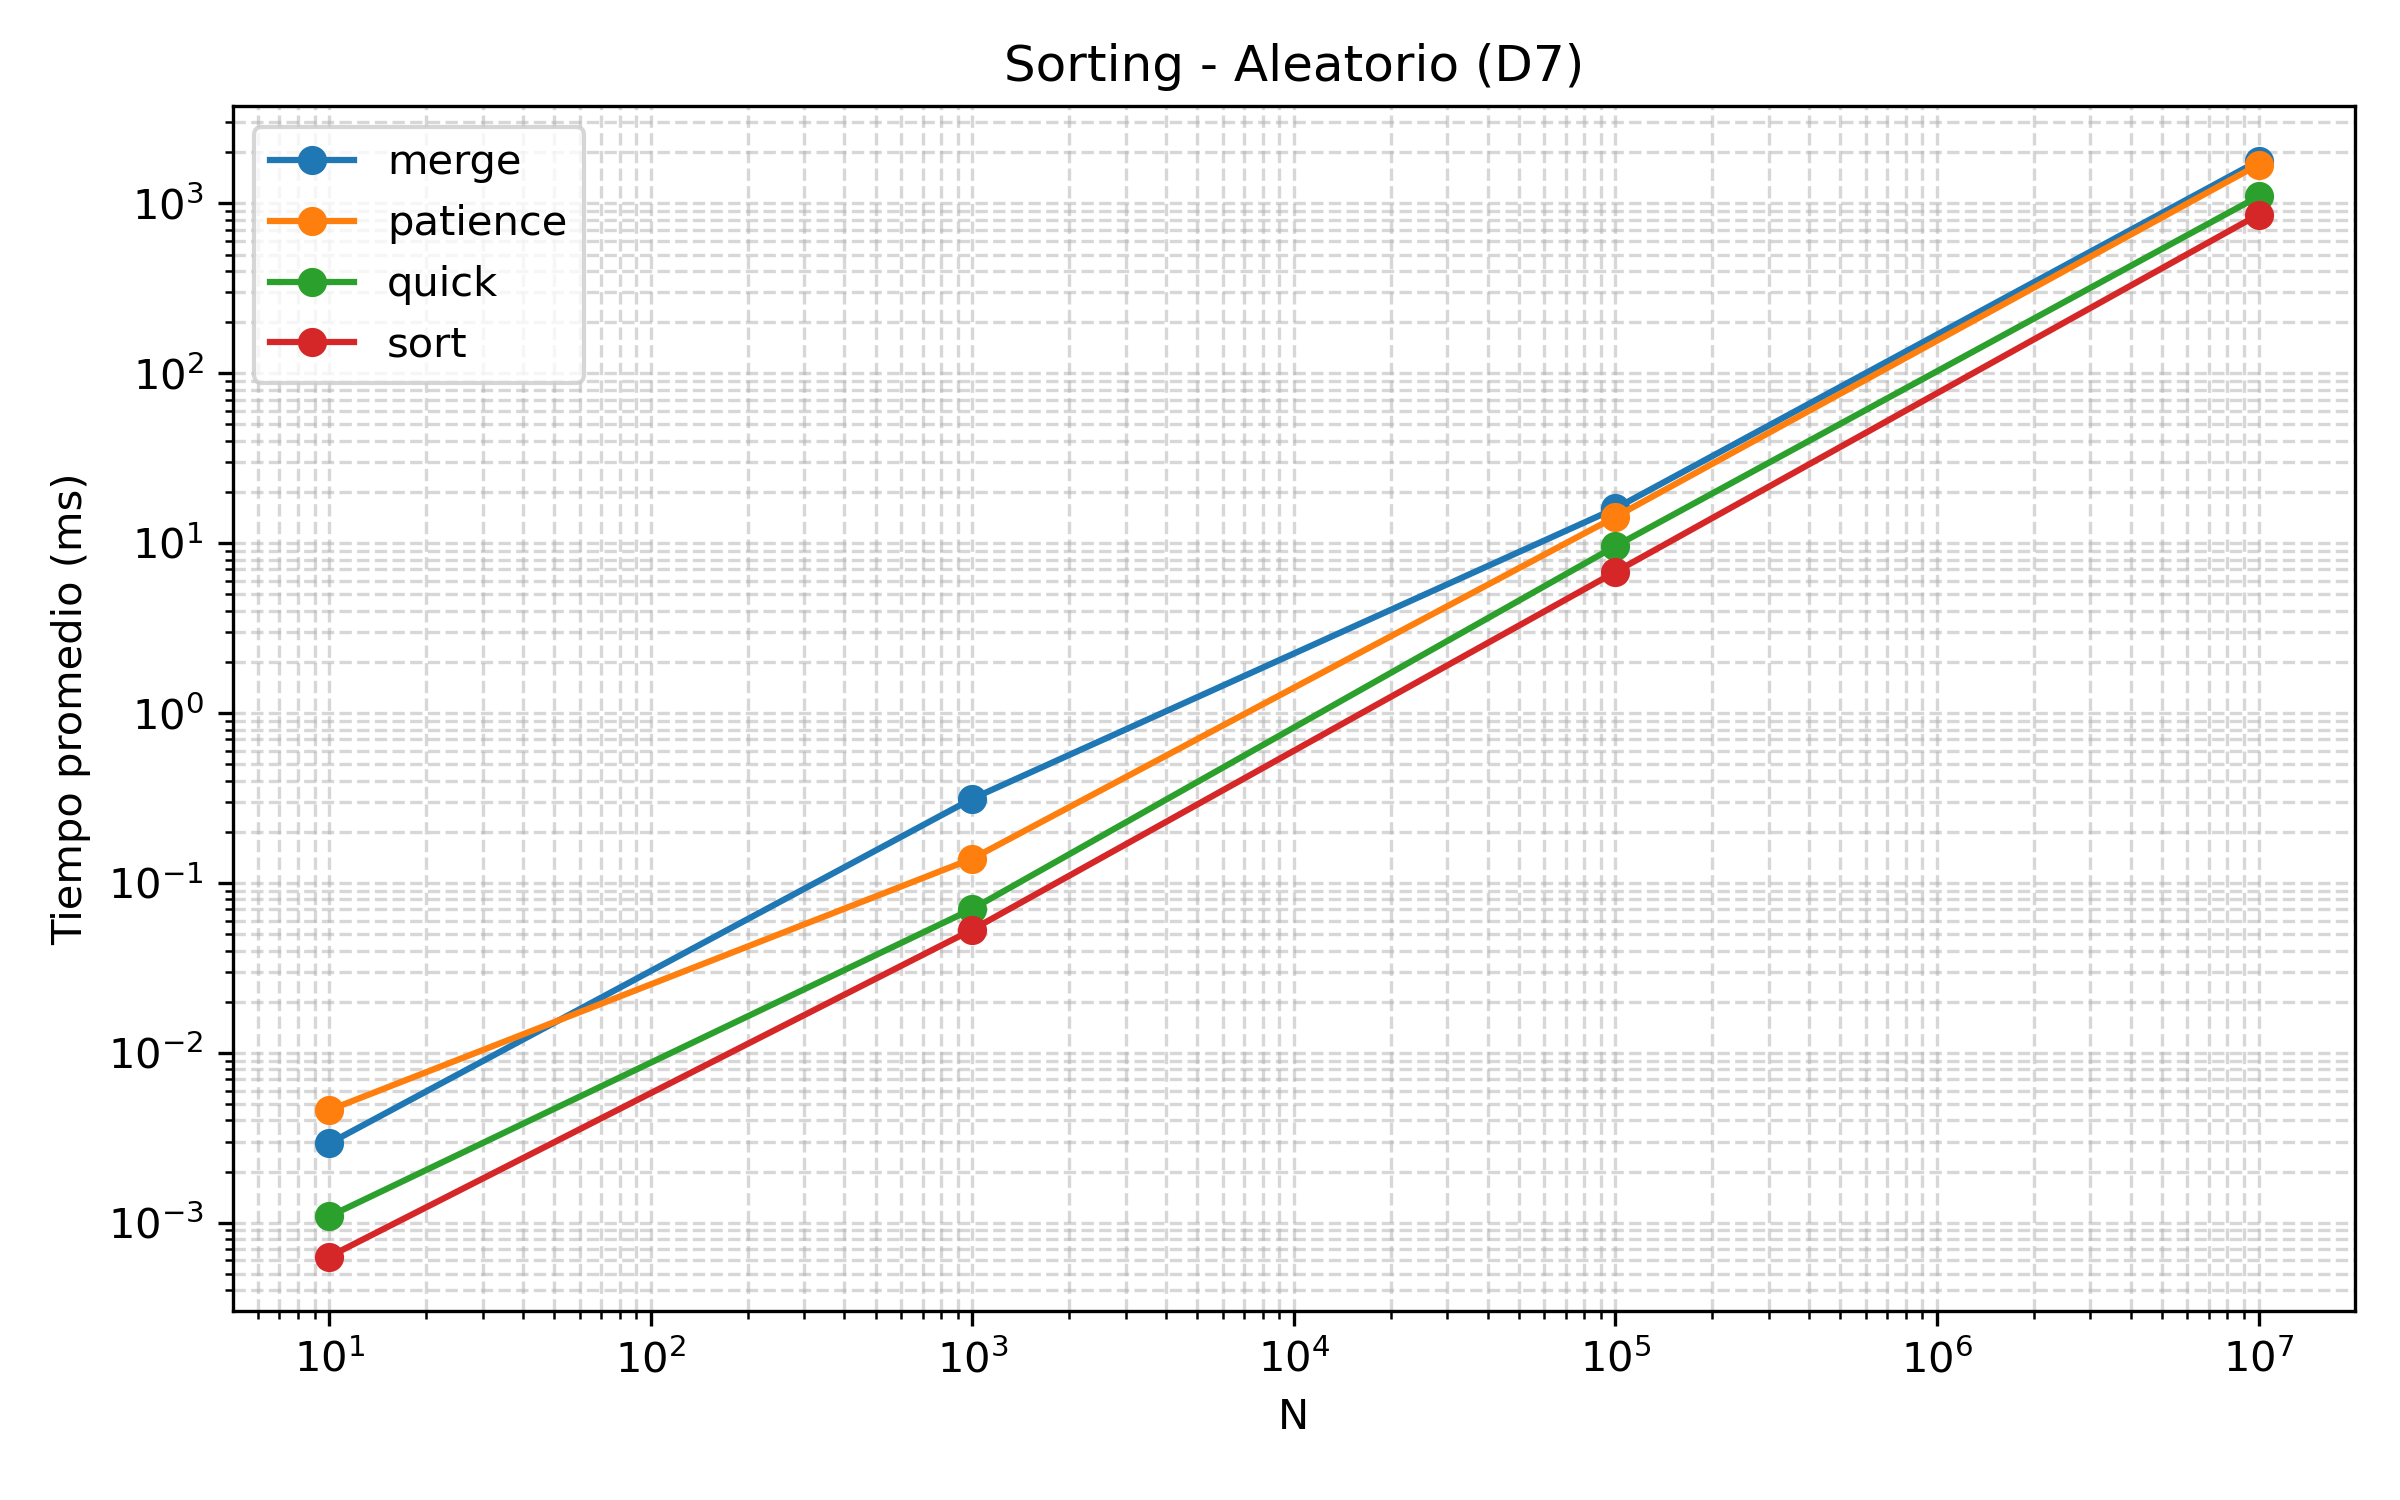
\includegraphics[width=\textwidth]{../code/sorting/data/plots/plot_aleatorio_D7.png}
        \caption{Caso promedio: entrada aleatoria ($D_7$).}
        \label{fig:sort_aleatorio_d7}
    \end{minipage}
    \hfill
    \begin{minipage}{0.48\textwidth}
        \centering
        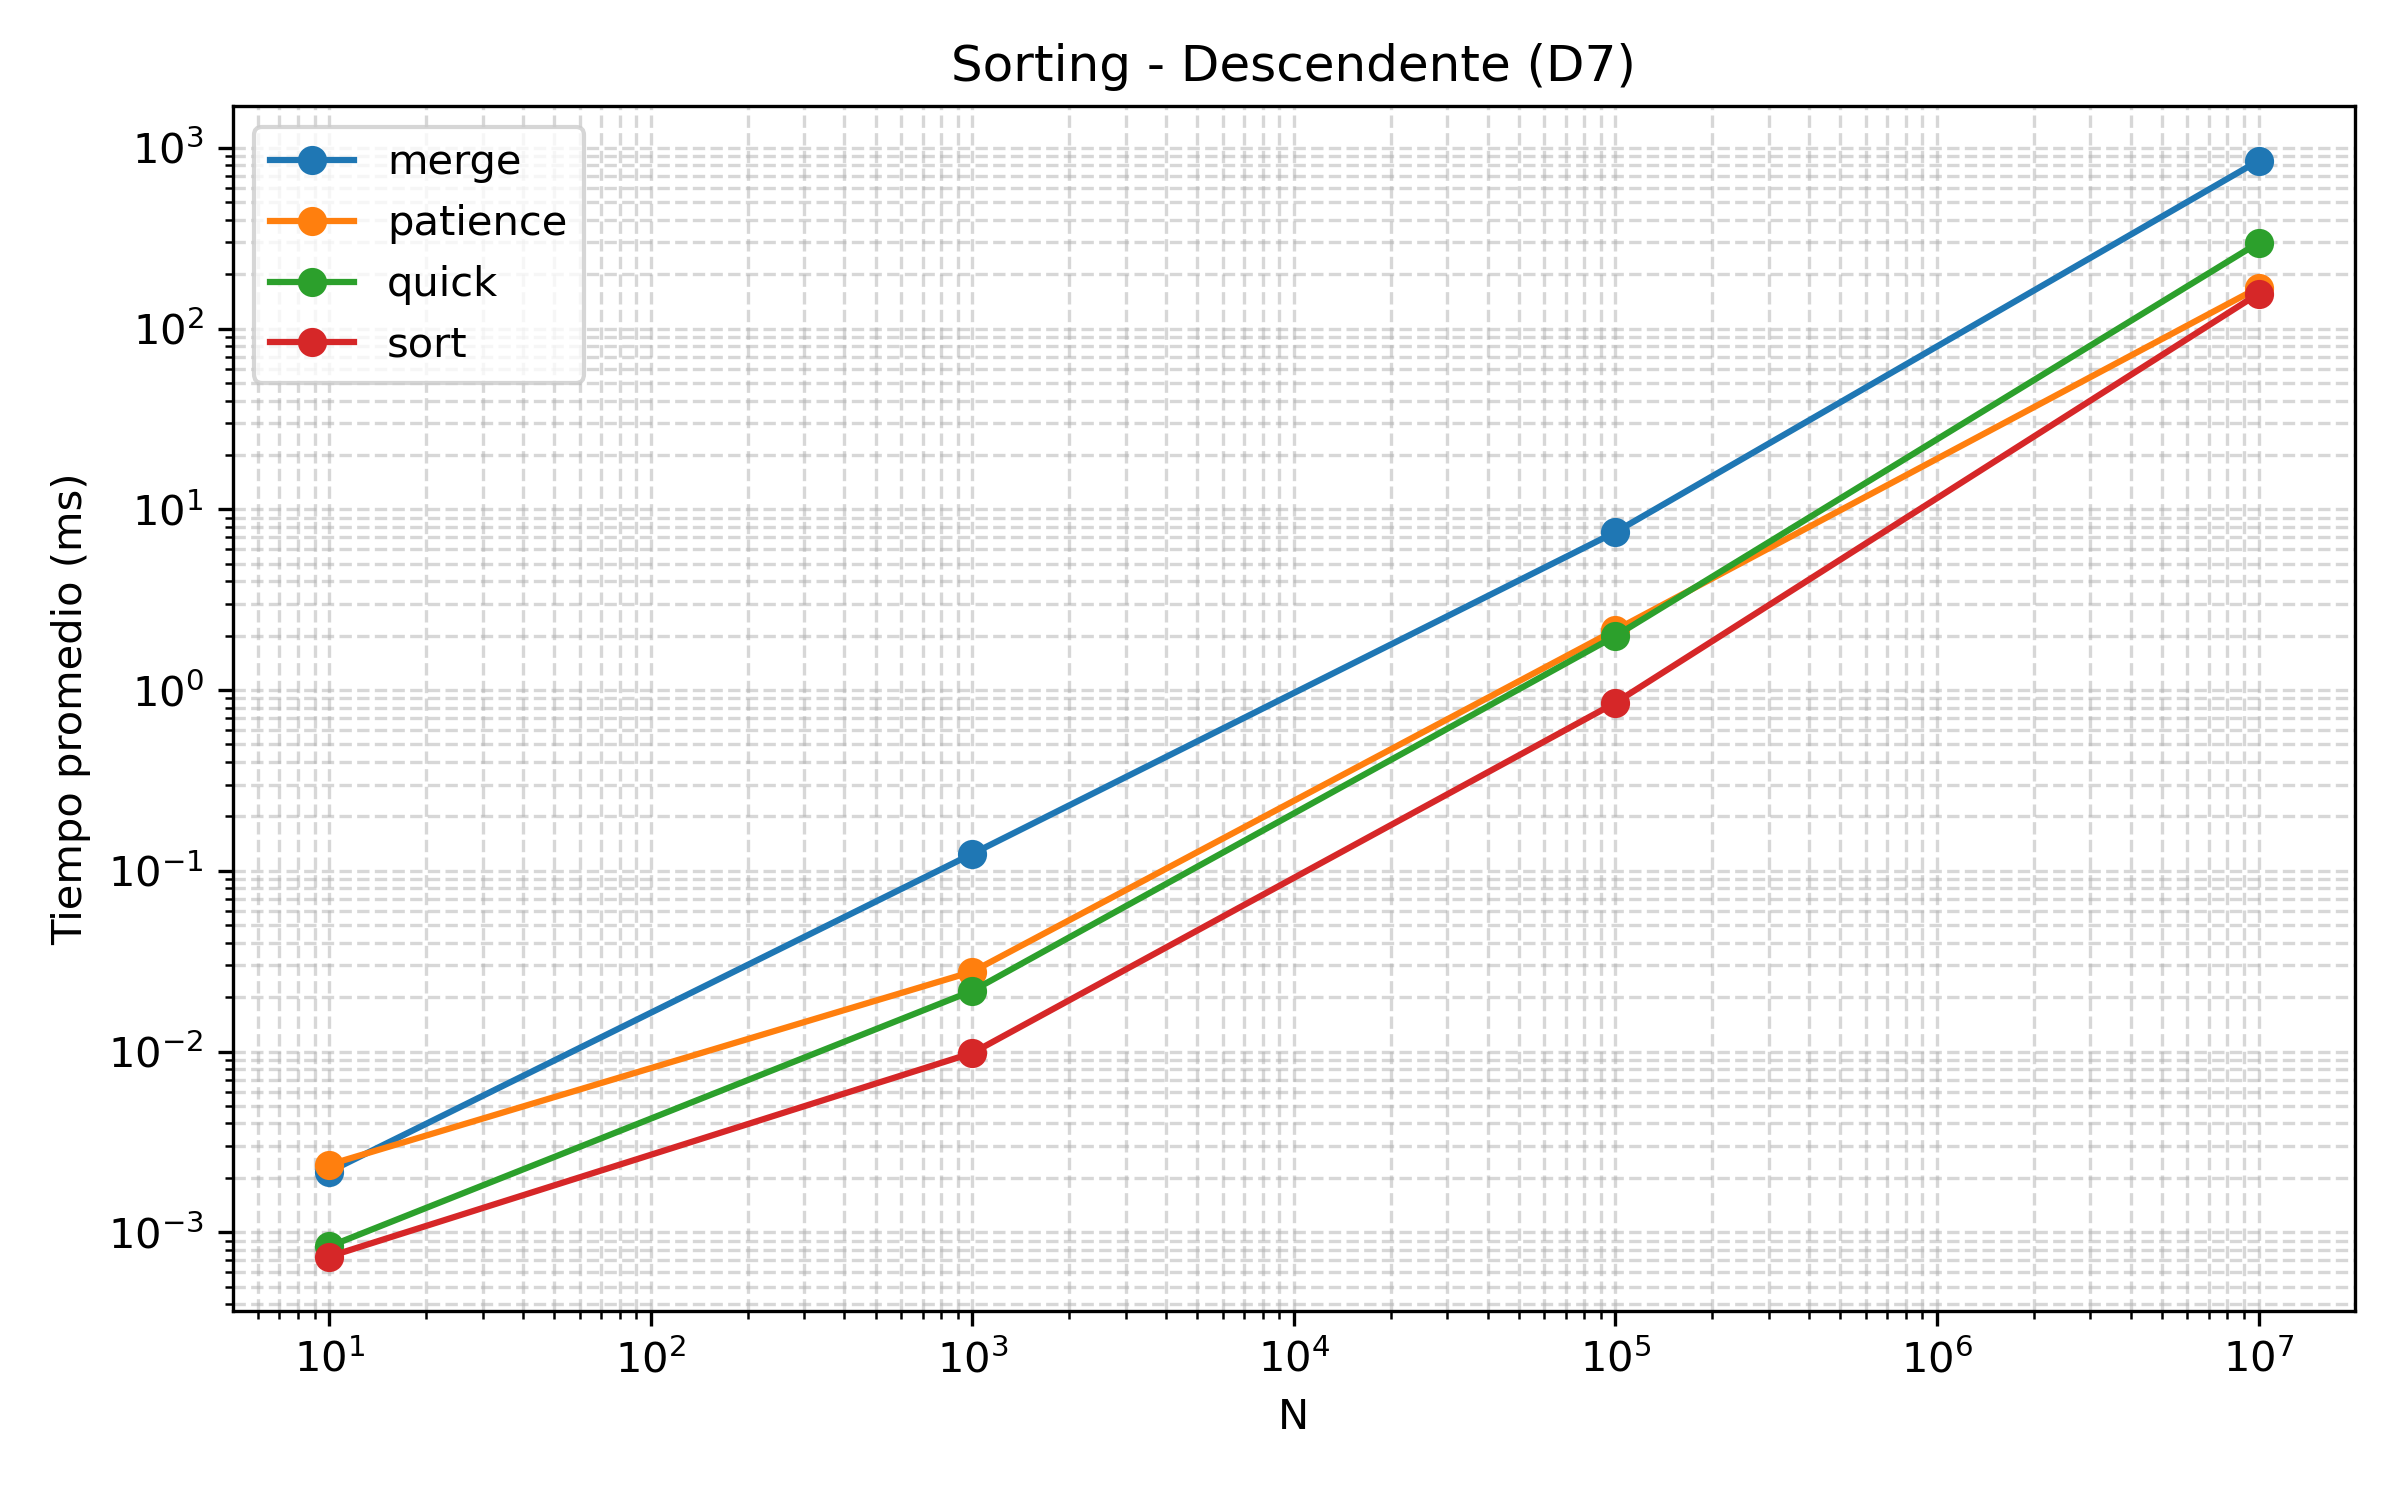
\includegraphics[width=\textwidth]{../code/sorting/data/plots/plot_descendente_D7.png}
        \caption{Mejor caso de Patience: descendente ($D_7$).}
        \label{fig:sort_descendente_d7}
    \end{minipage}
\end{figure}

En la Figura~\ref{fig:sort_aleatorio_d7} se presenta el comportamiento habitual con números desordenados. Como ambos ejes están en escala logarítmica (potencias de 10), una curva que se ve recta representa un crecimiento proporcional a su cota asintótica casi lineal $\mathcal{O}(N \log N)$. Podemos observar que:
\begin{enumerate}
    \item \textit{std::sort} y \textit{Quick Sort} lideran en velocidad. \textit{Quick Sort} implementa la partición de Hoare~\cite{educative_hoare_lomuto} (con dos punteros que recorren desde los extremos) y elimina la recursión de cola (usando un bucle para la mitad más grande), logrando tiempos muy cercanos a la biblioteca estándar de c++.
    \item \textit{Merge Sort} resulta más lento que los dos anteriores debido a la sobrecarga práctica de memoria: en cada paso recursivo necesita pedir memoria al sistema y copiar elementos a un arreglo auxiliar.
    \item \textit{Patience Sort} muestra tiempos mayores porque en una secuencia aleatoria se generan muchas pilas intermedias, exigiendo un esfuerzo continuo para insertar y extraer datos de su cola de prioridad.
\end{enumerate}

\begin{figure}[htbp]
    \centering
    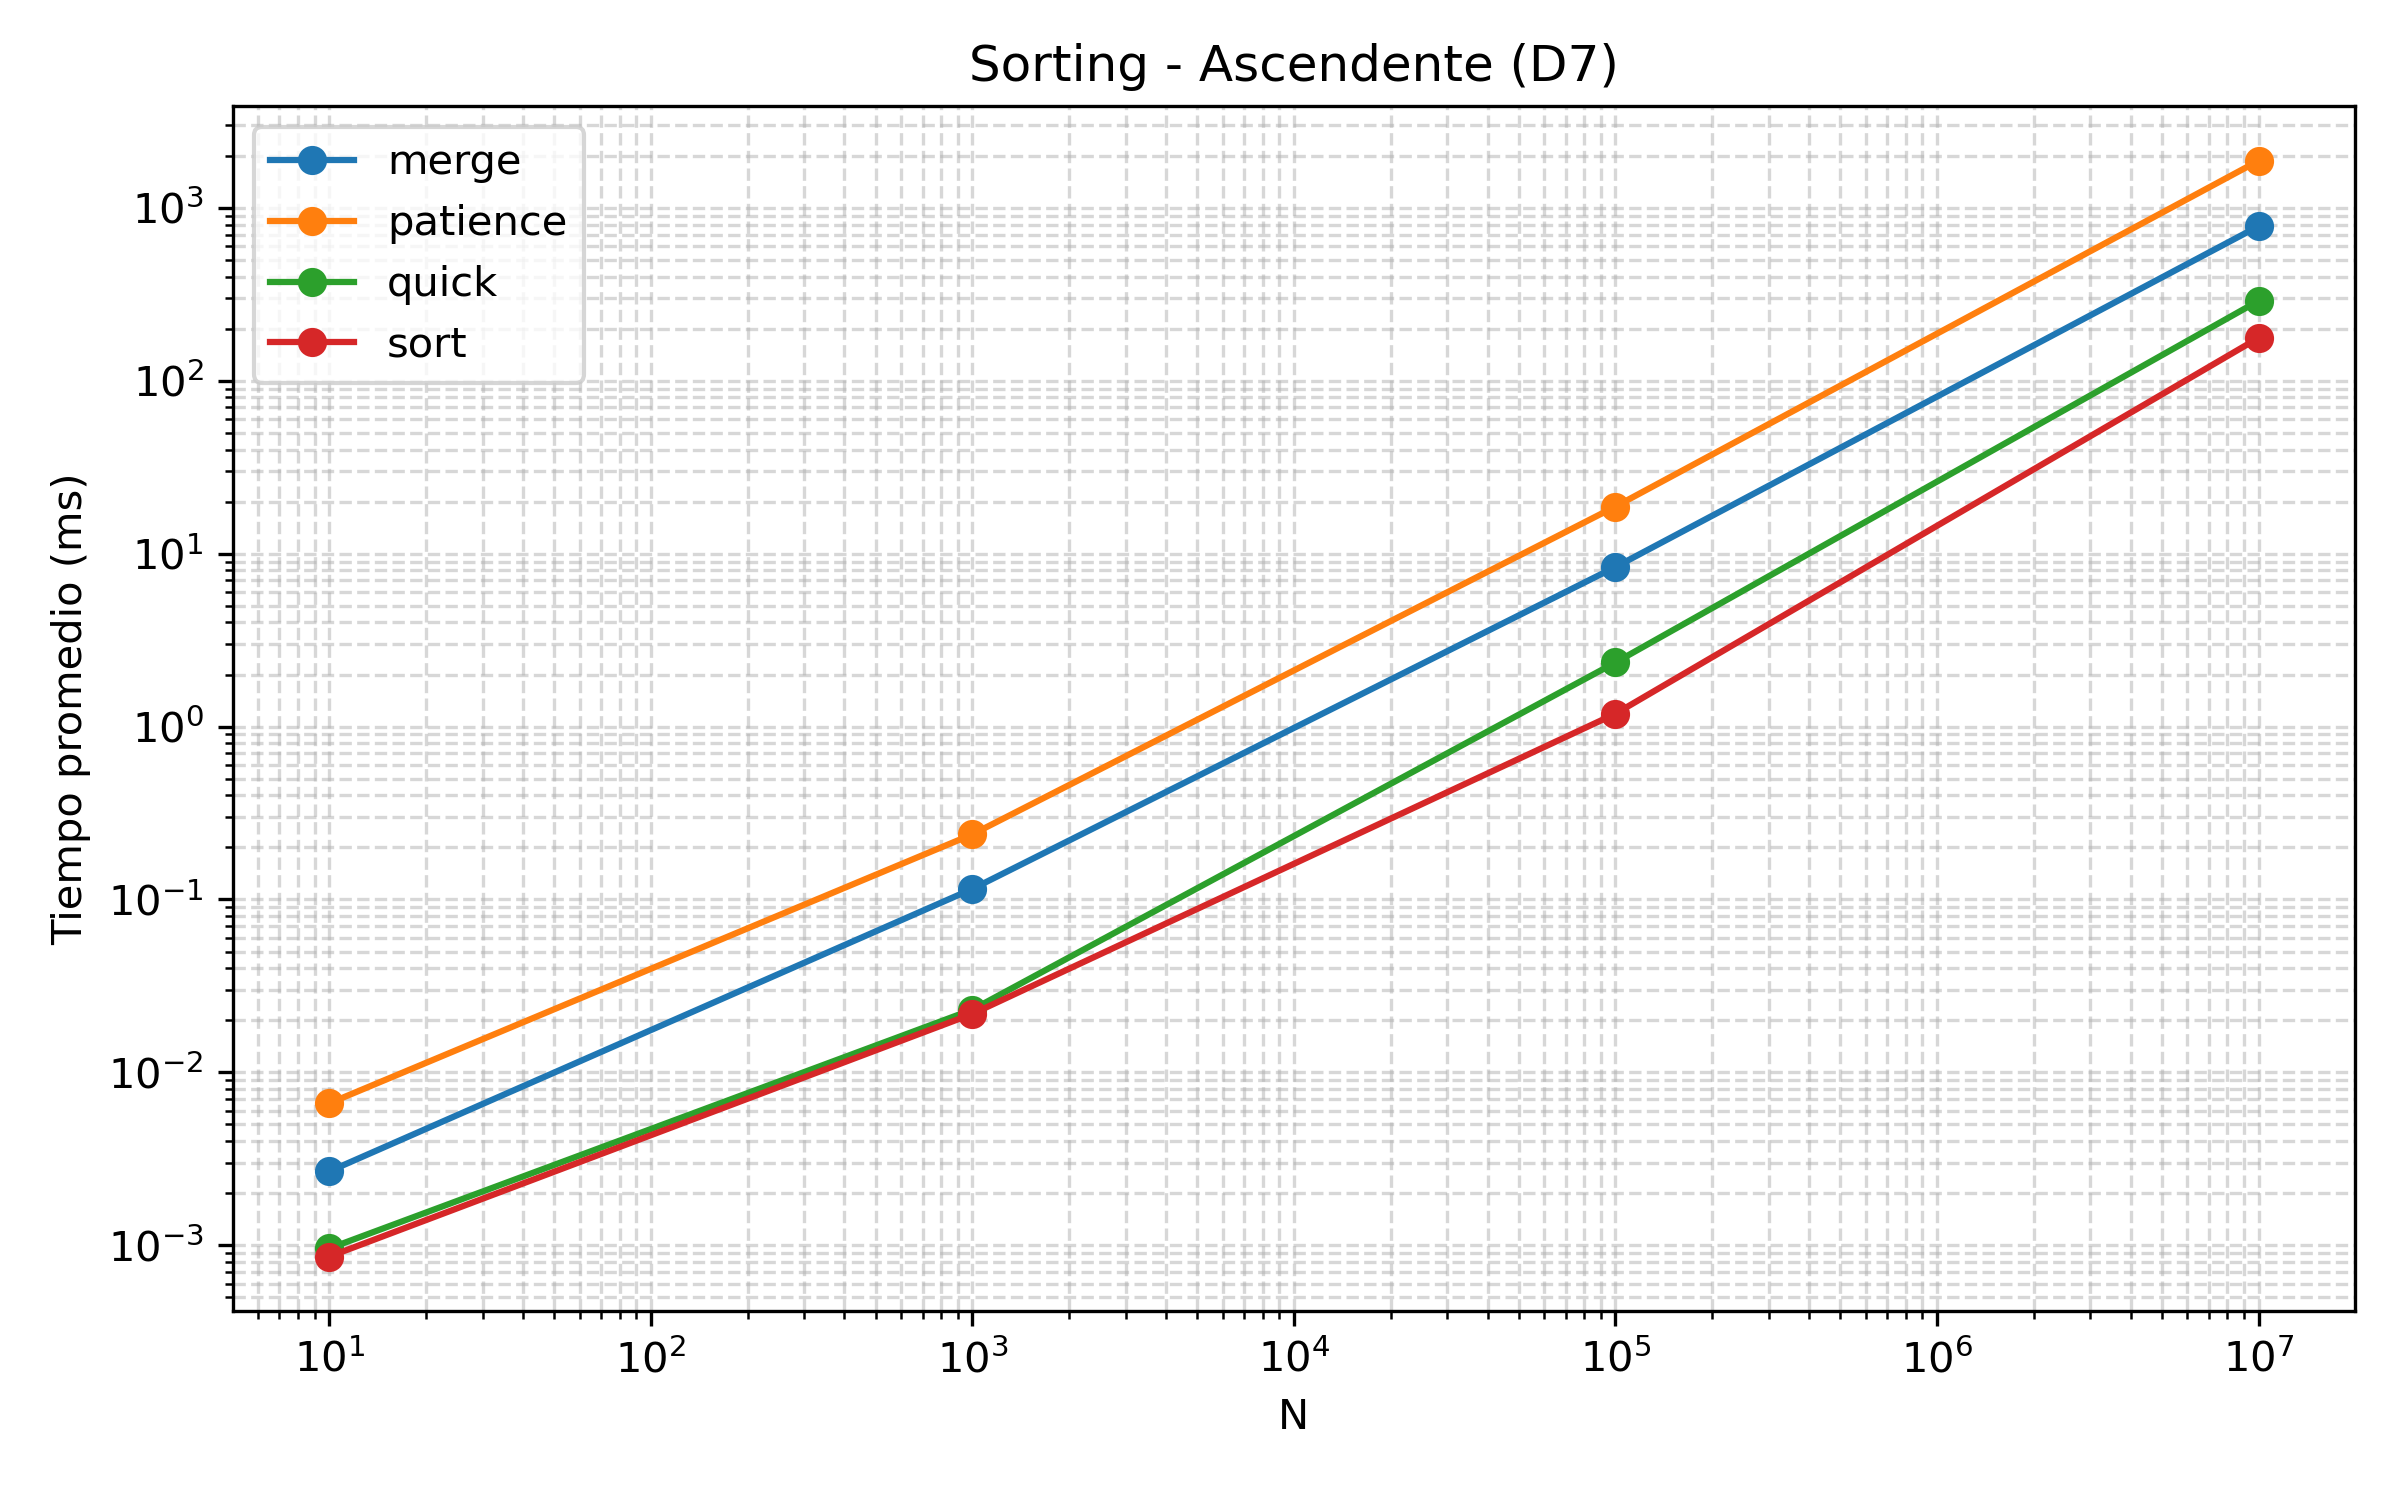
\includegraphics[width=0.55\textwidth]{../code/sorting/data/plots/plot_ascendente_D7.png}
    \caption{Peor caso de Patience: ascendente ($D_7$).}
    \label{fig:sort_ascendente_d7}
    \vspace{-0.5em}
\end{figure}

El contraste más revelador del experimento aparece al comparar las entradas ordenadas (Figuras~\ref{fig:sort_descendente_d7} y \ref{fig:sort_ascendente_d7}):
\begin{itemize}
    \item \textbf{La estabilidad de Quick Sort con esquema Hoare:} En la teoría clásica, cuando un arreglo ya está ordenado de forma ascendente o descendente, Quick Sort corre el riesgo de degradarse a un tiempo cuadrático $\mathcal{O}(N^2)$ si elige como pivote el primer o último elemento (pues divide el arreglo en un subarreglo de $N-1$ y otro vacío). En nuestras pruebas, la curva se mantiene completamente estable y rápida. Esto confirma el éxito de seleccionar el pivote en el punto medio del arreglo y usar el esquema de Hoare, balanceando las particiones evitando una ejecución que podría tardar incluso horas.
    \item \textbf{La notable asimetría de Patience Sort:} Este algoritmo funciona como el juego solitario de cartas: coloca cada nuevo número sobre la primera pila cuyo tope sea mayor o igual a él. 
    \begin{itemize}
        \item En la entrada \textbf{descendente} (Figura~\ref{fig:sort_descendente_d7}), cada nuevo número que llega es menor que el anterior, por lo que todos los elementos caen sucesivamente sobre una única pila ($k=1$). La etapa final de fusión con la cola de prioridad solo tiene que vaciar esa sola pila de principio a fin, logrando un tiempo casi lineal $\mathcal{O}(N)$ (su mejor caso posible).
        \item En la entrada \textbf{ascendente} (Figura~\ref{fig:sort_ascendente_d7}), cada nuevo elemento es más grande que todos los anteriores, por lo que nunca puede apilarse sobre ninguno y obliga a abrir una pila nueva por cada dato ($k=N$). La fase de reconstrucción tiene que gestionar un montículo de tamaño $N$, disparando el tiempo de ejecución hasta convertir a Patience Sort en el algoritmo más lento del benchmark para $N = 10^7$.
    \end{itemize}
\end{itemize}

\subsection{Resultados en Multiplicación Matricial}

Para la multiplicación de matrices cuadradas de $N \times N$, se comparó el algoritmo tradicional \textit{Naive} $\mathcal{O}(N^3)$ frente al método recursivo de \textit{Strassen} $\mathcal{O}(N^{2.807})$~\cite{bytequest2023strassen} para dimensiones $N \in \{16, 64, 256, 1024\}$ sobre dominios binarios ($D_0$) y enteros ($D_{10}$).

\begin{figure}[htbp]
    \centering
    \begin{minipage}{0.48\textwidth}
        \centering
        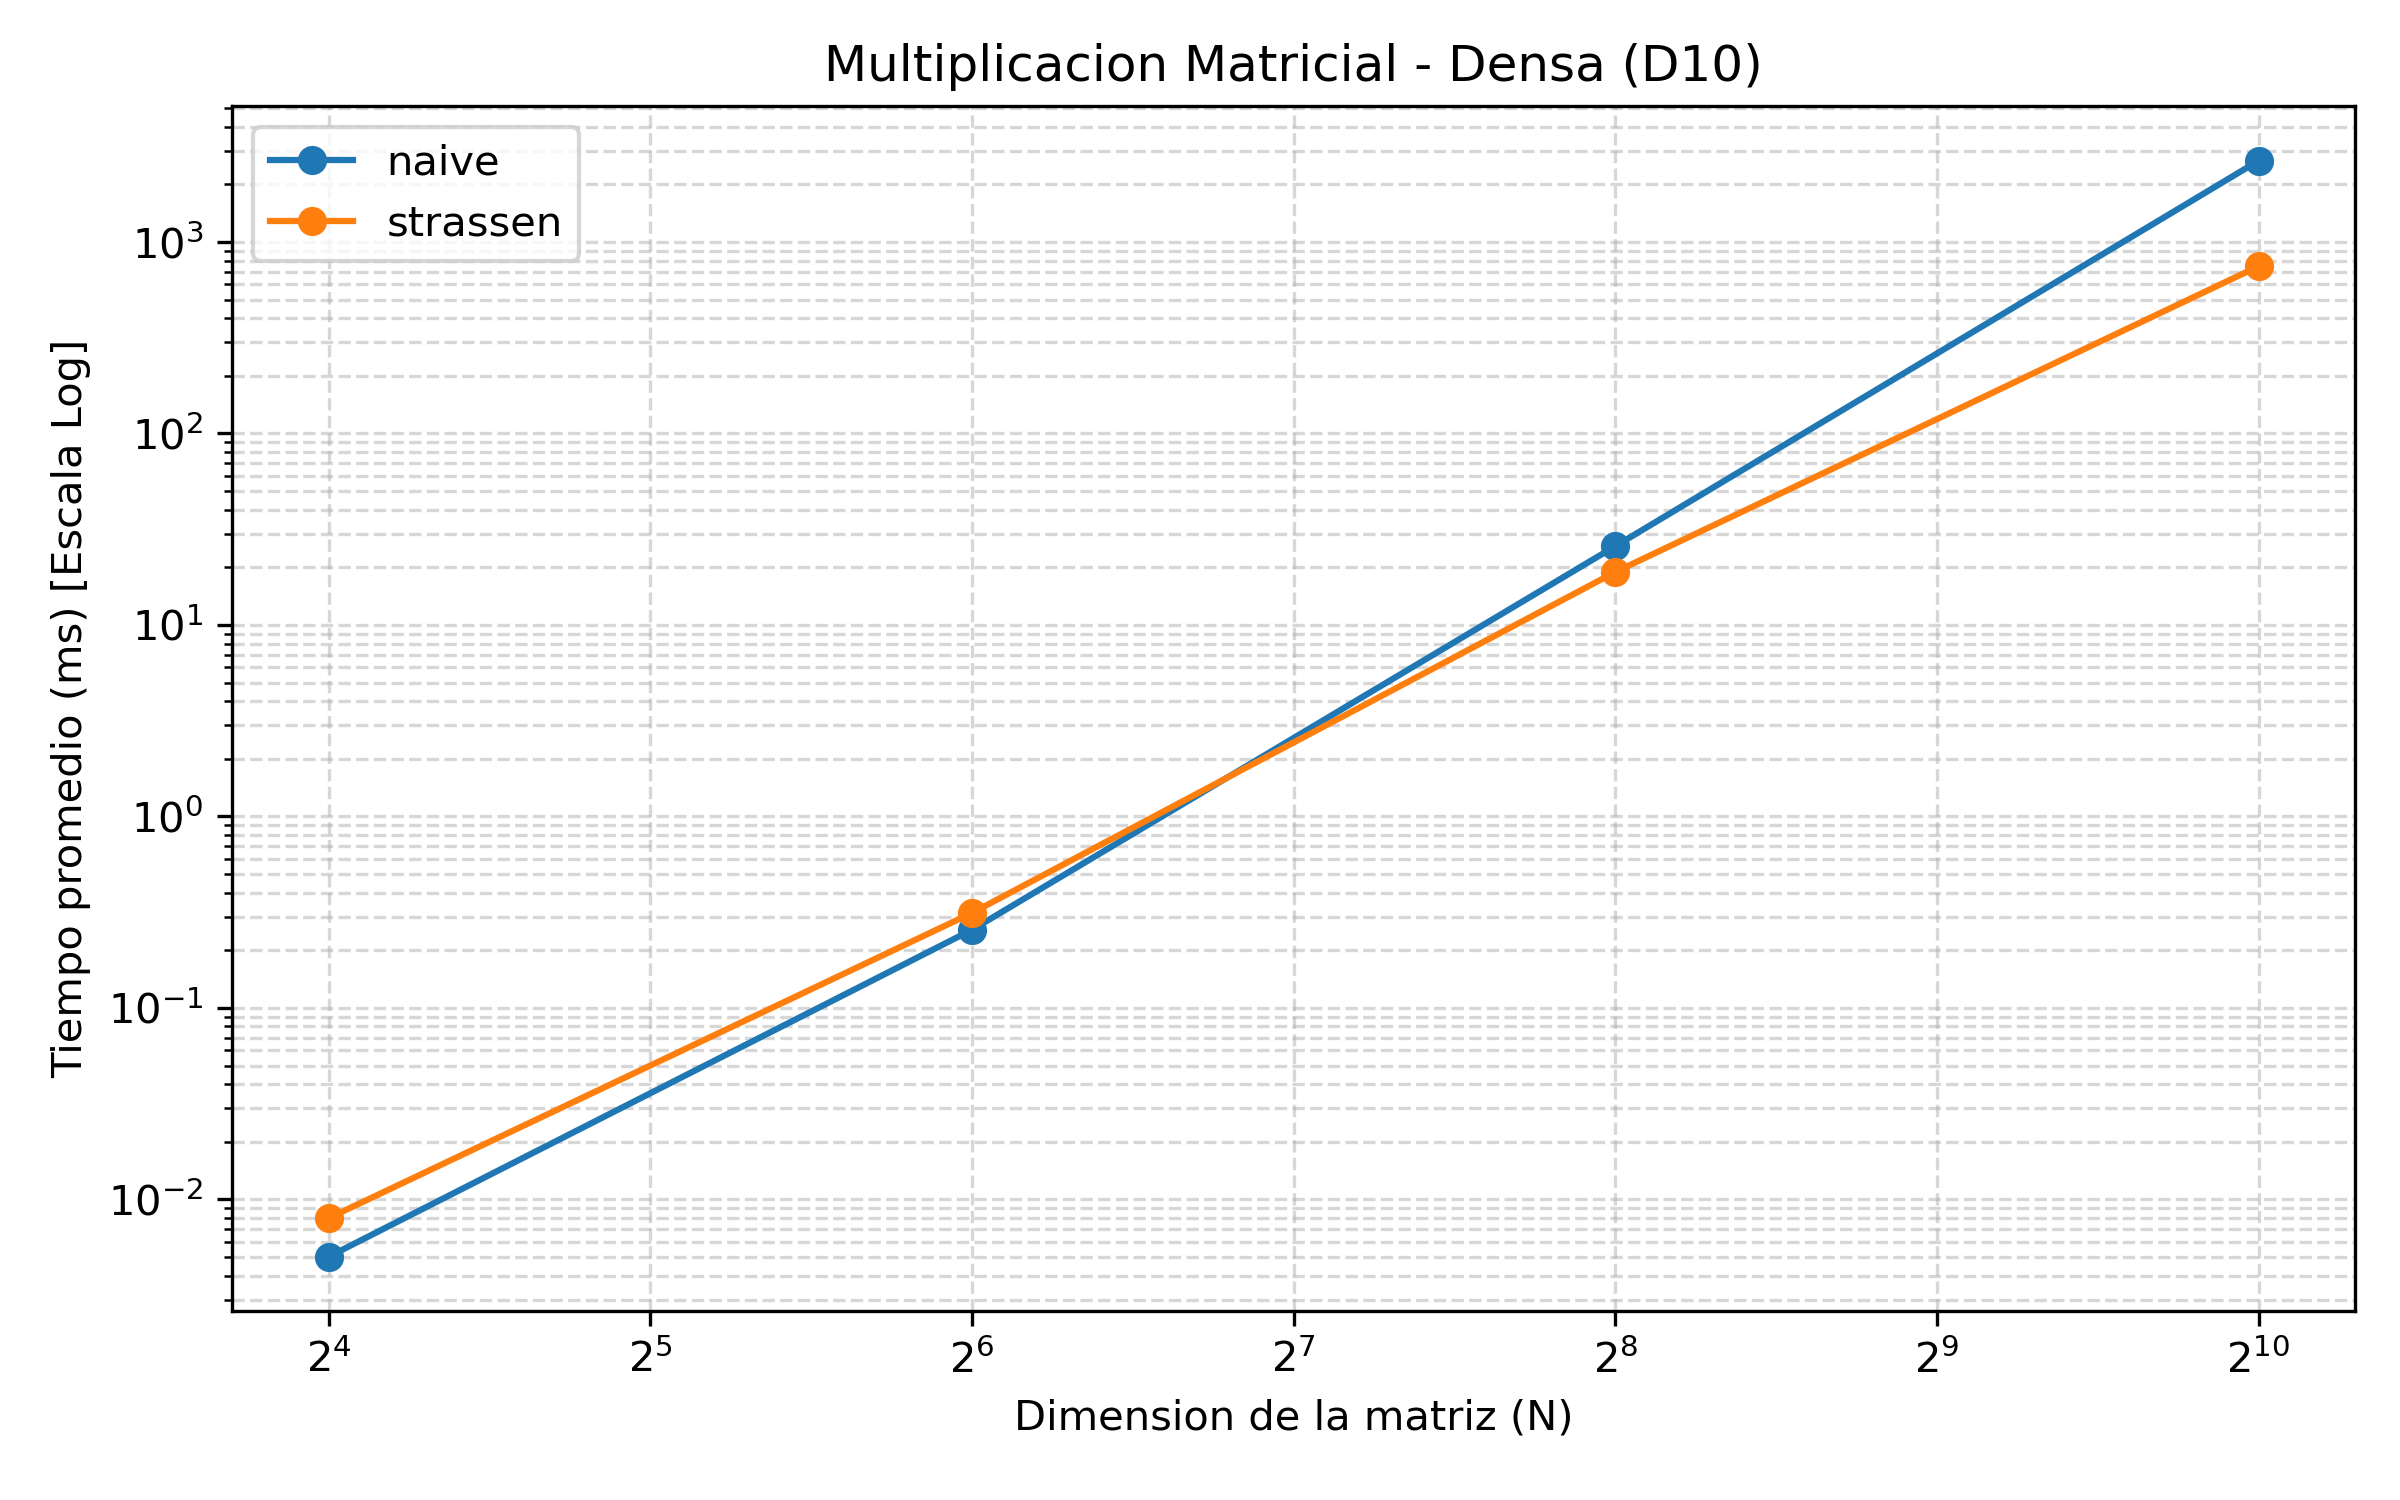
\includegraphics[width=\textwidth]{../code/matrix_multiplication/data/plots/plot_densa_D10.png}
        \caption{Multiplicación en matrices densas ($D_{10}$).}
        \label{fig:matrix_densa_d10}
    \end{minipage}
    \hfill
    \begin{minipage}{0.48\textwidth}
        \centering
        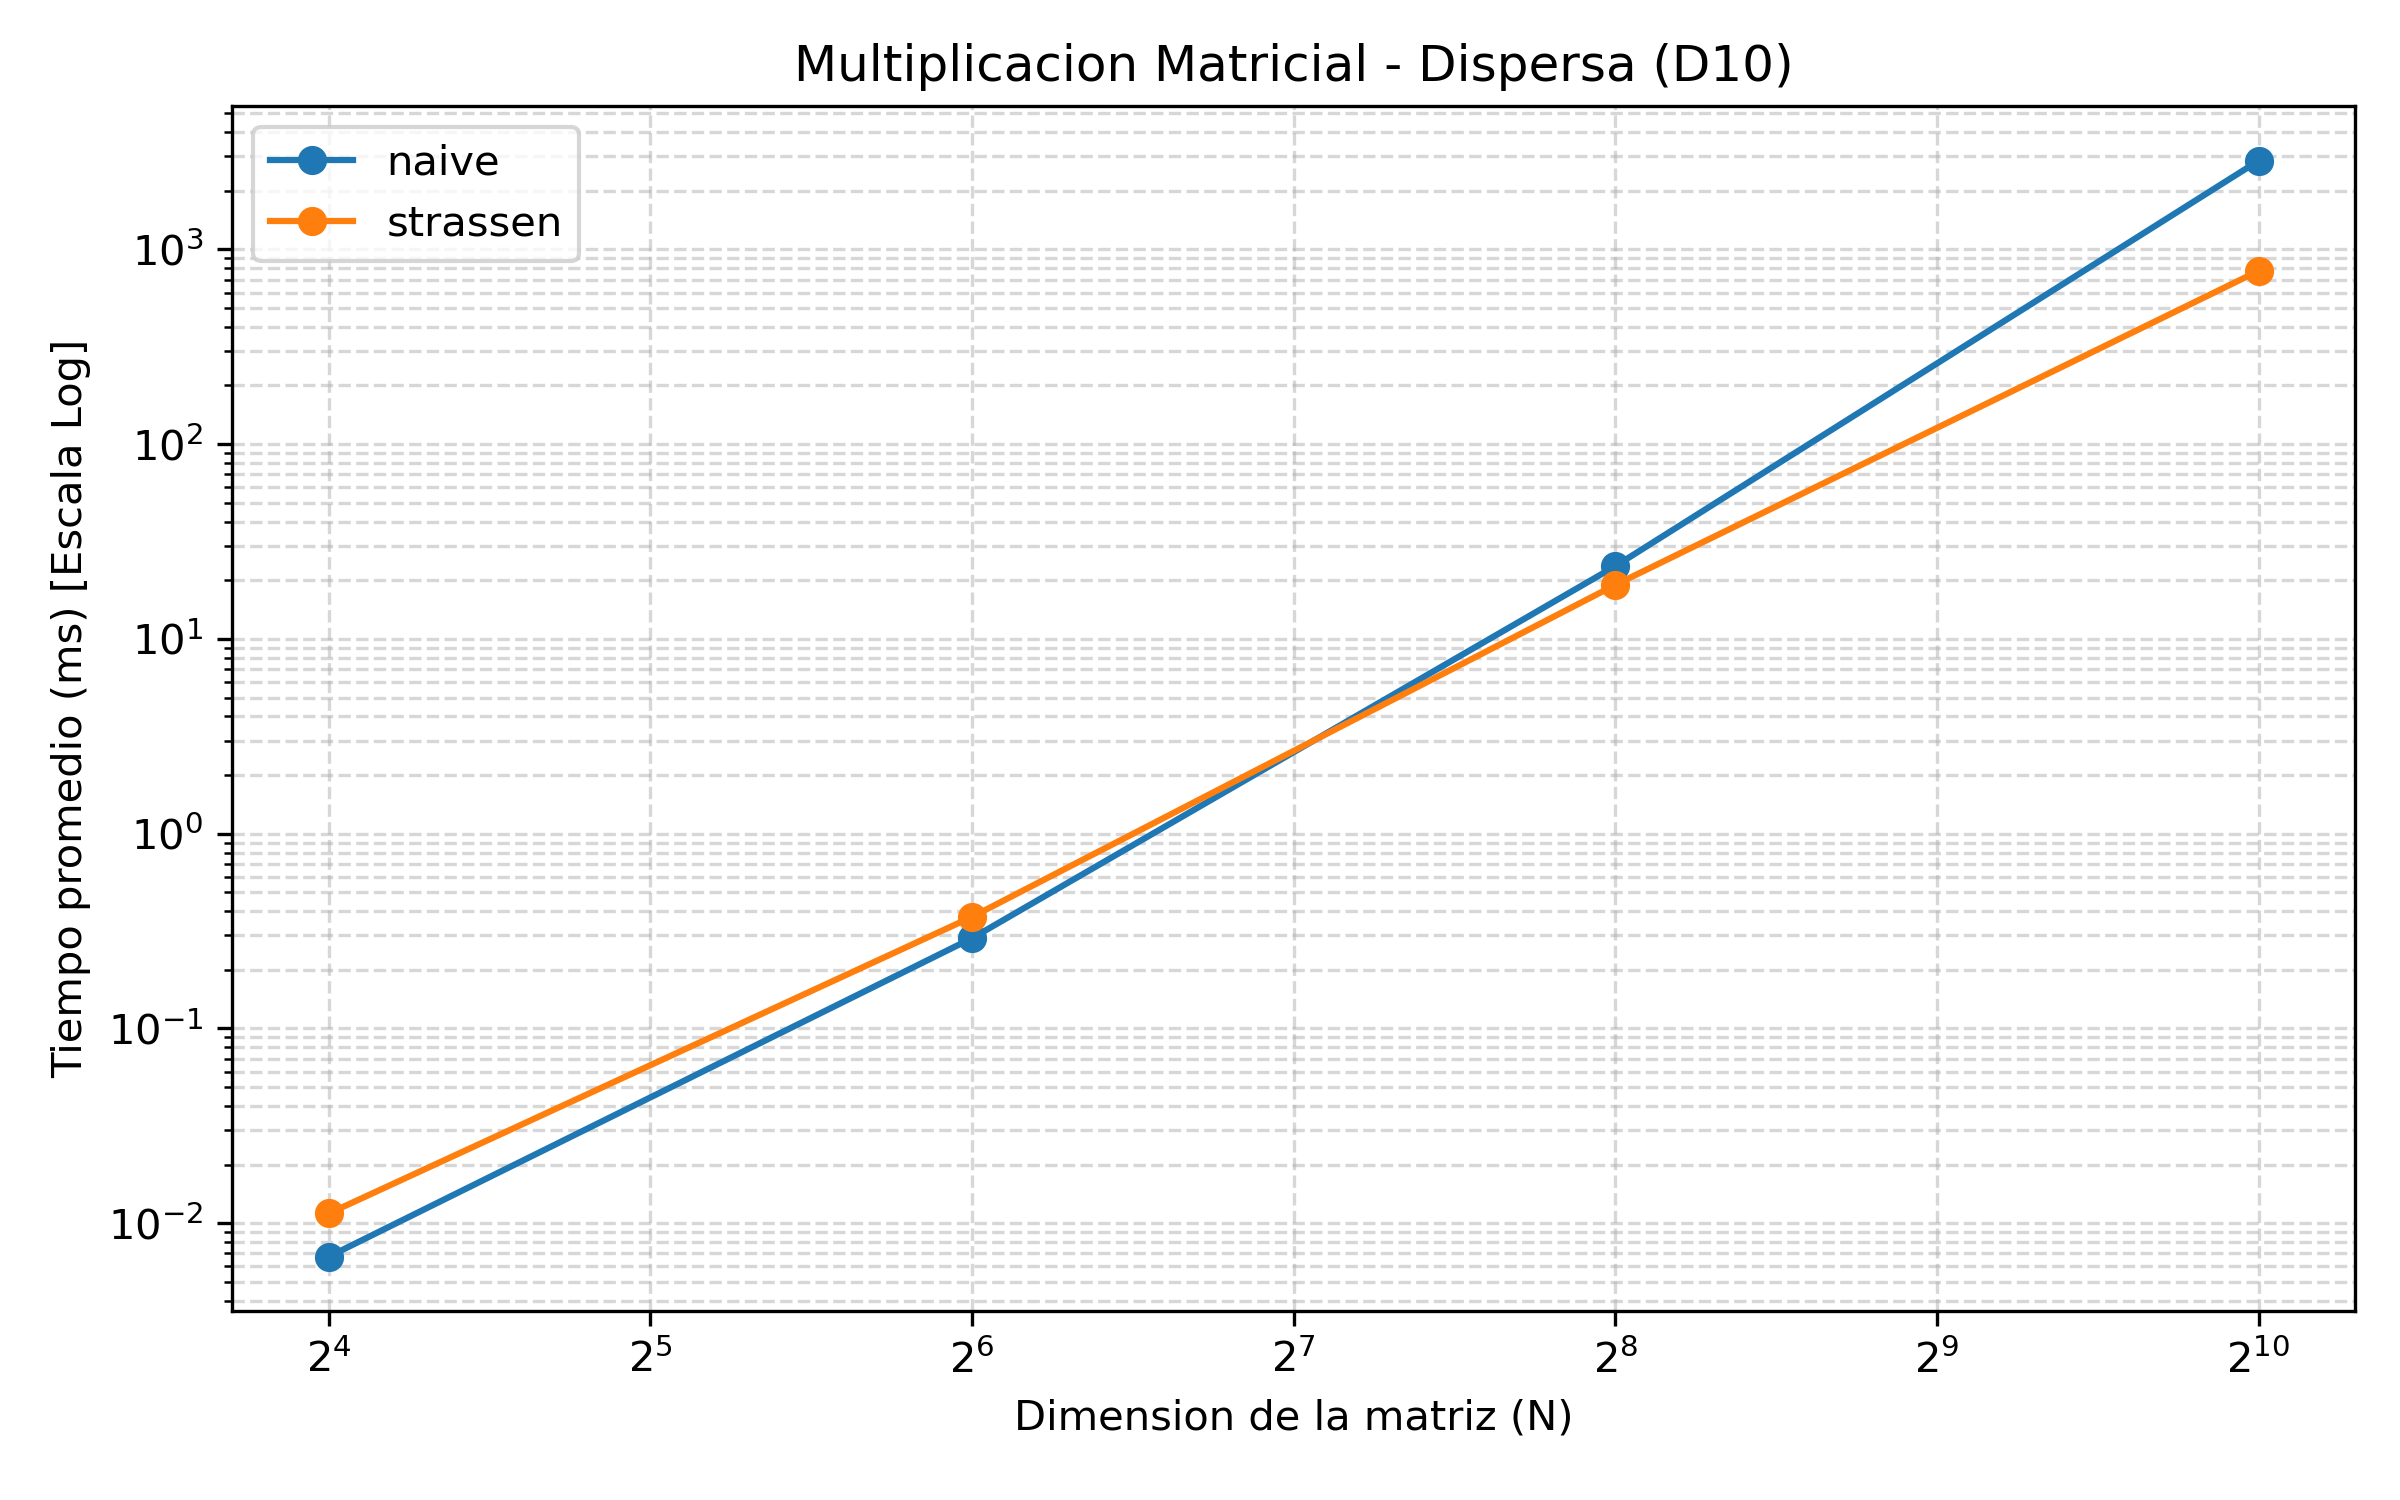
\includegraphics[width=\textwidth]{../code/matrix_multiplication/data/plots/plot_dispersa_D10.png}
        \caption{Multiplicación en matrices dispersas ($D_{10}$).}
        \label{fig:matrix_dispersa_d10}
    \end{minipage}
\end{figure}

En la Figura~\ref{fig:matrix_densa_d10} se observa claramente el compromiso entre constantes ocultas y cota asintótica:
\begin{enumerate}
    \item \textbf{Matrices pequeñas ($N \le 64$):} El algoritmo clásico \textit{Naive} supera en velocidad a Strassen. Esto ocurre porque la sobrecarga de crear submatrices temporales, realizar sumas matriciales y gestionar la recursión es mayor que el ahorro que ofrece calcular 7 multiplicaciones en lugar de 8.
    \item \textbf{Cruce asintótico ($N \ge 256$):} Al crecer la dimensión de las matrices, el término cúbico $N^3$ domina rápidamente. La menor pendiente asintótica de Strassen ($k \approx 2.81$) compensa la sobrecarga de memoria y reduce drásticamente el tiempo de ejecución para $N = 1024$.
\end{enumerate}

\begin{table}[htbp]
\centering
\caption{Resumen comparativo de complejidad teórica y comportamiento empírico.}
\label{tab:resumen_algoritmos}
\small
\begin{tabular}{|l|c|c|c|}
\hline
\textbf{Algoritmo} & \textbf{Complejidad Temporal} & \textbf{Complejidad Espacial} & \textbf{Sensibilidad a la Entrada} \\
\hline
Merge Sort & $\Theta(N \log N)$ & $\Theta(N)$ & Invariable ante el orden inicial \\
Quick Sort (Hoare) & $\mathcal{O}(N \log N)$ prom. & $\mathcal{O}(\log N)$ & Robusto con pivote central \\
Patience Sort & $\mathcal{O}(N \log k)$ & $\mathcal{O}(N)$ & Extrema (depende de la subsecuencia) \\
std::sort & $\mathcal{O}(N \log N)$ & $\mathcal{O}(\log N)$ & Invariable \\
\hline
Naive Matrix & $\mathcal{O}(N^3)$ & $\Theta(1)$ & Invariable ante ceros o densidad \\
Strassen & $\mathcal{O}(N^{2.807})$ & $\Theta(N^{2})$ & Invariable ante ceros o densidad \\
\hline
\end{tabular}
\end{table}

Por último, al comparar la Figura~\ref{fig:matrix_densa_d10} con la Figura~\ref{fig:matrix_dispersa_d10} (matrices dispersas al 10\%) y los casos de matrices diagonales, los tiempos de ejecución de ambos métodos son casi idénticos. Esto se debe a que las implementaciones utilizan una estructura de matriz densa estándar \texttt{std::vector$<$std::vector$<$int$>>$}, la cual itera y computa todas las posiciones sin realizar optimizaciones condicionales por la presencia de ceros.